\documentclass[aspectratio=169]{beamer}
\usetheme{Perso}

\usepackage[outputdir=build]{minted}
\setminted{breaklines}
\newminted{text}{frame=single}
\usemintedstyle{tango}
\graphicspath{ {images/} }

\title{The Lean Startup}
\date{\today}
\author{Maxime Vidori}

\begin{document}

\begin{frame}
  \titlepage
\end{frame}

\begin{frame}{Intro}
  \pause
  \LARGE \textbf{Why startups fail?} \normalsize \\
  \pause
\begin{block}{Achieving failure}
    Successfully, faithfully rigorously executing a plan that turned out to have
     been utterly flawed.
  \end{block}
  \pause
  \begin{block}{"Just do it" school of startups}
    If management is the problem , chaos is the answer!
  \end{block}


\end{frame}

\note[itemize]{
\item simple question -> Why startups fails
\item nothing was paved and no rules seamed to
}

\begin{frame}{Vision}{Define}
  \begin{itemize}
    \item who is an entrepreneur
    \item what is a startup (a 7000 people startup)
  \end{itemize}
\end{frame}

\begin{frame}{Vision}{Learn}
  \begin{itemize}
    \item measure
    \item validate learning
    \item value vs waste
    \item example IMVU: throw a lot of work away (plugin, pivot)
  \end{itemize}
\end{frame}

\begin{frame}{Vision}{Experiment}
  \begin{itemize}
      \item think big, start small
      \item an experiment is a product.
      \item validate hypothesis
  \end{itemize}
\end{frame}

\note{
build, measure, learn feedback loop
}

\begin{frame}{Steer}
  \begin{figure}
    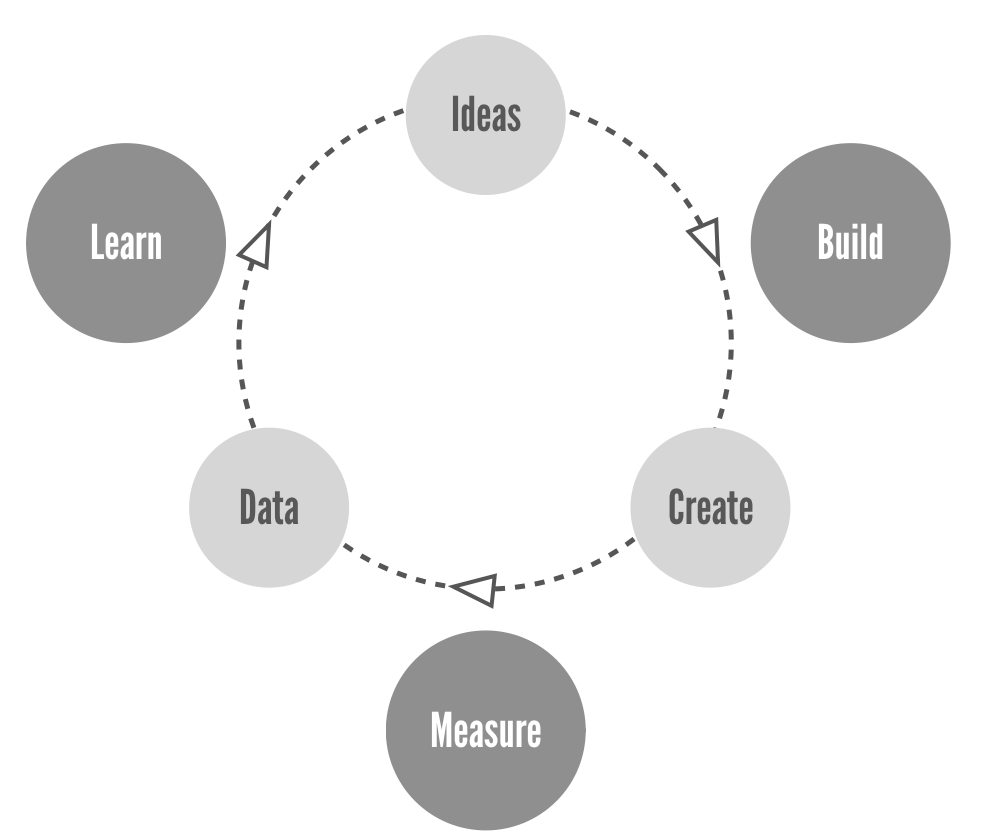
\includegraphics[scale=0.24]{build-measure-learn}
  \end{figure}
\end{frame}


\begin{frame}{Steer}{Leap}
  \begin{itemize}
    \item strategy based on assumptions
    \item beyond "The right place at the right time"
    \item value and growth
    \item Genchi Gembuchu
    \item analysis paralysis
  \end{itemize}
\end{frame}

\begin{frame}{Steer}{Test}
  \begin{itemize}
    \item Well known MVP's
      \begin{itemize}
        \item Groupon
        \item Dropbox
      \end{itemize}
    \item Different types of MVPs
      \begin{itemize}

        \item video minimum viable product
        \item concierge MVP
        \item wizard of Oz MVP
      \end{itemize}
    \item Early adopters!
  \end{itemize}
\end{frame}

\begin{frame}{Steer}{Measure}
  \begin{itemize}
    \item Three learning milestone
      \begin{itemize}
        \item establish the baseline
        \item tuning the engine
        \item pivot or persevere
      \end{itemize}

    \item ! Vanity metrics -> product progress =/= business results
    \item cohort analysis
    \item actionable metrics
  \end{itemize}
\end{frame}

\begin{frame}{Steer}{Pivot or Persevere}
  \begin{itemize}
    \item startup runway (number of pivots left)
    \item pivot or persevere meeting
  \end{itemize}
\end{frame}

\begin{frame}{Accelerate}{Batch}
  \begin{itemize}
    \item Continuous Deployment
    \item Large batch death spiral
    \item Andon cord
  \end{itemize}
\end{frame}

\begin{frame}{Accelerate}{Grow}
  \begin{itemize}
    \item where does it come from -> three engines of growth
  \end{itemize}
\end{frame}

\begin{frame}{That's all folks}
  \LARGE \textbf{Questions?}

  \begin{flushright}
    \normalsize github.com/\color{Green}IxDay\color{Grey}/talks/the-lean-startup
   \end{flushright}
\end{frame}


\end{document}
